%-----------------------------------------------------------%
% Propuesta de plantilla en LaTeX para tesis formato UAG    %
% Autor: Arnulfo Moisés Maciel Hernández                    % 
% Contacto: moy.maciel@gmail.com                            %
% Fecha: Septiembre 2017                                    %
%-----------------------------------------------------------%
% El objetivo de esta plantilla es facilitar la redacción   %
% en LaTeX de tu tesis siguiendo los lineamientos de la UAG.%
% Mi intención es pues que se dedique el tiempo al          %
% contenido de la tesis evitando las largas horas           %
% entendiendo LaTeX.                                        %  
% Siéntete libre de modificar la plantilla de acuerdo a tus %
% necesidades.                                              %
%-----------------------------------------------------------%
% Utiliza el libro libro LaTeX_2014.pdf que se encuentra    %
% dentro de la carpeta "ayuda" para más información.        %
%-----------------------------------------------------------%

%-----------------------------------------------------------%
% Las siguientes configuraciones son con el objetivo de una
% tesis en español siguiendo los lineamientos estipulados
% en: http://crecea.uag.mx/opciones/tesis.htm
% En relación al diseño de la portada los lineamientos 
% estipulados en: http://crecea.uag.mx/opciones/portada.htm

    \documentclass[12pt,twoside]{report}
    \usepackage[utf8]{inputenc}
    % Incluye la bibliografia en el indice general
    \usepackage[nottoc]{tocbibind}              
    \usepackage{pdfpages}
    \usepackage{longtable,multirow,booktabs}
    \usepackage{setspace}
    \usepackage{graphicx}
    \usepackage{cite}
    \usepackage{tabu}
    \usepackage[spanish, es-tabla]{babel}
    \usepackage{amssymb}
    \usepackage{amsmath}
    \usepackage{esvect}
    \usepackage{hyperref}
    \usepackage[a4paper,width=150mm,top=25mm,bottom=25mm,bindingoffset=6mm]{geometry} %Formato márgenes, etc.
    \usepackage[font=footnotesize,labelfont=bf]{caption}
    \usepackage{minted}
    \usepackage{tikz}
    \usepackage{verbatim}
    \graphicspath{{imagenes/}} %Ubicación de imágenes
    \hypersetup{
        %Configuración comandos de referencia cruzada en LATEX:
        colorlinks=true,
        linkcolor=black,
        citecolor=blue,
        filecolor=blue,      
        urlcolor=blue,
        %Opciones de visualización e información PDF:
        pdfauthor={"Salvador Gudiño Ochoa"},
        pdftitle={"Modelado y Desarrollo de la herramienta eduintegral para la generación de un canal de comunicación padre de familia maestro"},
        pdfsubject={"Canal de comunicación para maestros y alumnos"},
        pdfcreator={"Salvador Gudiño Ochoa"},
        pdfproducer={"Salvador Gudiño Ochoa"},
        pdfkeywords={""}
    }
    
    \begin{document}
    
        %Carátula de tesis

\begin{titlepage}
    \begin{center}
        \rule{\textwidth}{4pt}\vspace*{-\baselineskip}\vspace*{2pt} % Thick horizontal line
        \rule{\textwidth}{1pt}\\[\baselineskip] % Thin horizontal line
        \textbf{\normalsize UNIVERSIDAD AUTÓNOMA DE GUADALAJARA} % Title
        \rule{\textwidth}{0.4pt}\vspace*{-\baselineskip}\vspace{3.2pt} % Thin horizontal line
        \rule{\textwidth}{1.6pt}\\[\baselineskip] % Thick horizontal line
        
        {\tiny CON RECONOCIMIENTO DE VALIDEZ OFICIAL DE ESTUDIOS DE LA SECRETARÍA DE \\ EDUCACIÓN PÚBLICA SEGÚN ACUERDO No.158 DE FECHA 17 DE JULIO DE 1991} % Title
        \rule{\textwidth}{0.4pt}\vspace*{-\baselineskip}\vspace{3.2pt} % Thin horizontal line
        \rule{\textwidth}{1.6pt}\\[\baselineskip] % Thick horizontal line

        \textbf{\small POSGRADOS EN COMPUTACIÓN} % Title
        
        \vspace*{1.2cm}
        
\includegraphics[width=0.3\textwidth]{uag_2.jpg}
        \vspace*{1.2cm}
        
        {\small Modelado y Desarrollo de la herramienta Eduintegral para la generación de un canal de comunicación padre de familia maestro}
        \rule{\textwidth}{0.6pt}\\[\baselineskip] % Thick horizontal line
        
        \textbf{\small PROYECTO DE INTERVENCIÓN} % Title
        \vspace*{1.2cm} 
        
        {\scriptsize QUE PRESENTA}
        
        \textbf{\scriptsize Salvador Gudiño Ochoa }
        \vspace*{1.2cm}
        
        {\scriptsize PARA OBTENER EL GRADO DE}
        
        \textbf{\small MAESTRÍA EN CIENCIAS COMPUTACIONALES} % Title
        \vspace*{1.2cm}
        
        {\scriptsize ASESOR:\\ Dr. Jonathan Hernando Rosales Hernández}
        
        \vspace*{1.2cm}
        %\vfill % Esto pone hasta el final la siguiente linea p0ps
        
        {\scriptsize GUADALAJARA, JALISCO. Agosto 2019 }
        %\\ Número de registro en el sistema de investigación}
        \rule{\textwidth}{4pt}\vspace*{-\baselineskip}\vspace*{2pt} % Thick horizontal line
    \end{center}
\end{titlepage}
    
        %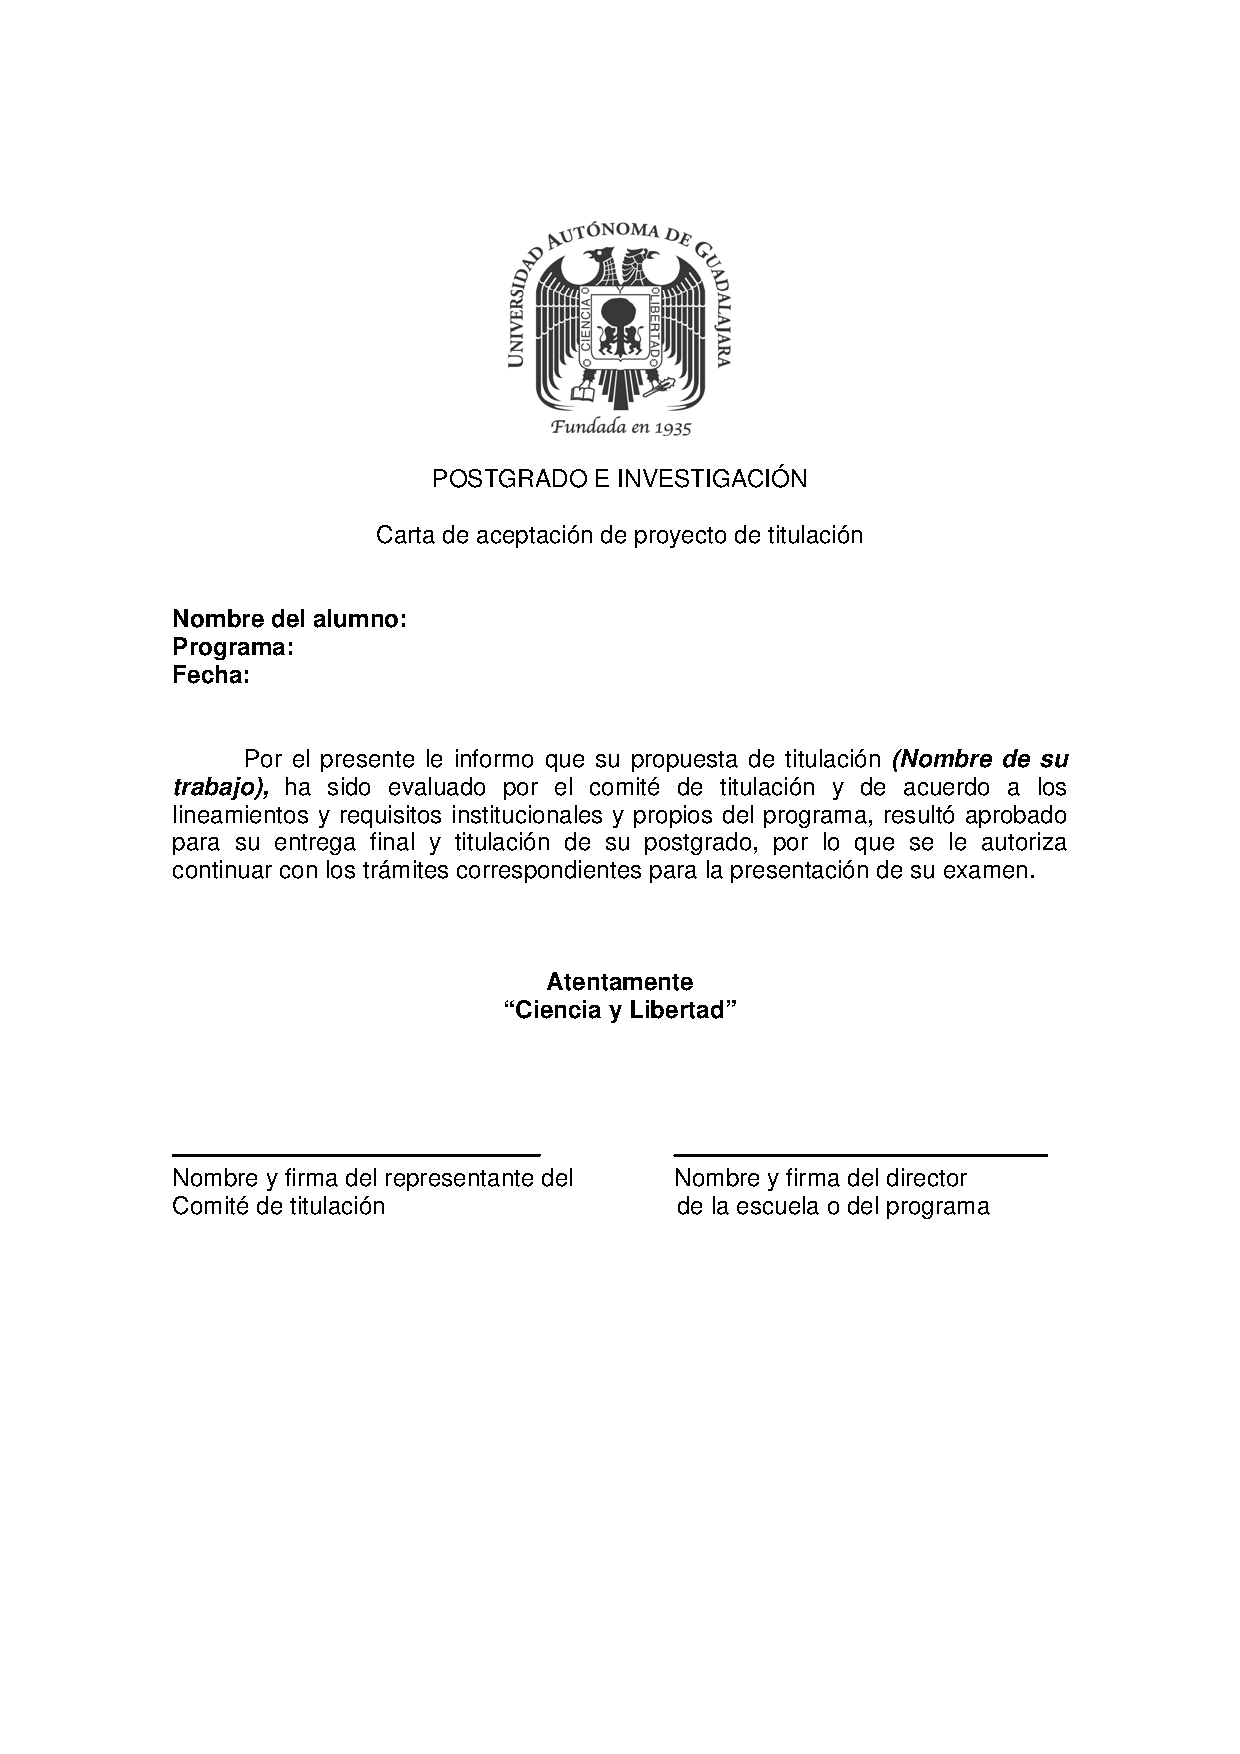
\includepdf[]{portada/cartaaceptacion.pdf} %archivo PDF y nombre de tu carta de aceptación % Removido por mi p0ps
        
         % Usar numeros romanos
        \pagenumbering{roman}
        
        \spacing{1.5}
        %\chapter*{Abstract}  % Removido por mi p0ps
        %%Abstract

El presente documento se ha elaborado con la finalidad de mostrar un ejemplo ilustrativo genérico, sin embargo se podrá elegir otros modelos de acuerdo a las características del programa académico y en concordancia con el director.
“La tesis tiene la opción de realizarse en forma interdisciplinaria, siempre y cuando se justifique de acuerdo al alcance del proyecto y en conformidad con las áreas correspondientes.” \cite{einstein}. 
 % Removido por mi p0ps
        

        \chapter*{Agradecimientos y dedicatoria}
        %Dedicatoria

Dedico este trabajo a todas las personas que esten interesadas en leer este trabajo y en extraer el conocimiento que les sea útil, ya que para mi particular punto de vista este tipo de trabajos existe solo con el propósito de promover el conocimiento adquirido durante mi estancia en la maestría de ciencias computacionales y así aportar un poco al crecimiento de las personas interesadas en este ámbito.

Aprovecho también para agradecer a todas las personas involucradas en mi vida que me ayudaron durante mi paso por la maestría de ciencias computacionales en la Universidad Autóname de Guadalajara.
        \addcontentsline{toc}{chapter}{Agradecimientos y dedicatoria}
        
        \chapter*{Resumen}
        %Resumen

En el ambiente estudiantil existe un reto de mejorar la comunicación que hay entre padres de familia y maestros. Usualmente, cuando el desempeño academico del alumno disminuye los padres de familia son informados una vez que este ya se encuentra bajo, no estan siendo informados en el momento oportuno para prevenir que el desempeño de su hijo baje. Si se mejora la comunicación entre padres de familia y maestro mediante la creación de un canal de comunicación directo e inmediatio esto ayudaria enormemente a los padres de familia a darse cuenta del desempeño del hijo sin tener que esperar hasta ver al maestro. Actualmente las aplicaciones que pueden ser adquiridas en México estan orientadas en la mejora de la labor del maestro, no como tal en la mejora de la comunicación entre padres de familia y maestros para lograr la mejora del desempeño del alumno. Dentro del alcance de este proyecto se propone el modelado y desarrollo de la aplicación móvil Eduintegral \cite{eduintegral}, la cual se pretende sea una poderosa herramienta que sea facilitadora del trabajo realizado por los maestros pero más importante sea el motor para mejorar la comunicación entre los padres de familia y los maestros, a través del uso de notificaciones inmediatas generadas por los maestros hacia los padres de familia. Esto será realizado tomando como partida el estado actual de Eduintegral \cite{eduintegral} y desarrollandolo al punto de que sea una aplicación que pueda ser utilizada en campo, para lo que se mejorará su arquitectura teniendo como enfoque un sistema distribuido, centrado en datos y multiplataforma.
        \addcontentsline{toc}{chapter}{Resumen}
        
        \chapter*{Summary}
        % Summary

In the scholar environment there is a challenge to improve communication between parents and teachers. Usually, when the student's academic performance decreases parents are informed once their child's performance is already low, they are not being informed in a timely manner to prevent their child's student performance from going down. If communication between parents and teacher is improved by creating a direct and immediate communication channel this would greatly help parents realize their child's performance without having to wait until they go with the teacher. Currently the applications that can be acquired in Mexico are aimed at improving the work of the teacher, not as such in improving communication between parents and teachers to achieve the student performance improvement. Within the scope of this project, the modeling and development of the mobile application Eduintegral \cite{eduintegral} is proposed, which is intended to be a powerful tool that will facilitate the work done by teachers but more important is the engine to improve communication between parents and teachers, through the use of immediate notifications generated by teachers to parents. This will be done taking as a starting point the current state of Eduintegral \cite{eduintegral} and developing it to the point that it is going to be an application that can be used in the field, for which its architecture will be improved taking into account a distributed system, focus on data and multiplatform.
        \addcontentsline{toc}{chapter}{Summary}
        
        \tableofcontents
        
        \listoffigures
        
        \listoftables 
         
        \cleardoublepage
        % Usar numeros arabicos
        \pagenumbering{arabic}
        
        \chapter{Introducción}
        %Capítulo 1

    El desempeño del estudiante en el día a día en México esta directamente relacionado al nivel de comunicación que tienen los actores principales en el ambiente educativo, los cuales son:
    
    \begin{itemize}
        \item El maestro
        \item El alumno
        \item Los padres de familia
    \end{itemize}
    
    Estos actores tienen que tener una buena comunicación para mantener el desempeño del alumno en un nivel satisfactorio. \\ El desempeño estudiantil en México es medido de manera cuantitativa y cualitativa, se requiere que el alumno tenga una buena conducta lo cuál se mide con la cantidad de reportes que pueda tener o no el alumno, en cuánto a la asistencia a clases, el alumno tiene que asistir al menos un 80\% del total de las clases y finalmente las calificaciones que son númericas marcan si el alumno tiene grado aprobatorio en el ciclo escolar vigente.


    \section{Descripción del problema} \label{descripcionproblema}
    
        Los padres de familia no están involucrados de manera constante en la educación de sus hijos, en consecuencia cuando un padre de familia recibe la información del desempeño de su hijo sucede con un retardo considerable, usualmente cuando ya es demasiado tarde y no hay manera de revertir el problema en el ciclo escolar en el que ocurrio. \\ Hay que remarcar que existen señales que nos indican cuando un alumno está teniendo un mal desempeño academico, esto no sucede de un dia a otro, por lo tanto si estas señales se detectan a tiempo y son resueltas oportunamente el desempeño del alumno puede mantenerse la mayor parte del tiempo favorable. \\ Precisamente, esta problemática es la que se intenta solventar en este proyecto, el problema de que practicamente la comunicación entre los padres de familia y los maestros es muy limitada, lo cual tiene como efecto colateral la afectación del desempeño del alumno.


    \section{Motivación del proyecto} \label{motivacionproyecto}

        La tecnología a crecido colosalmente en las últimas décadas a puntos que jámas hubieramos imaginado hoy en día, este crecimiento se ve reflejado en México y en el mundo, es por ello que esta es una gran época para los ingenieros de software que son capaces de aprovechar las herramientas que ofrecé la industria y el conocimiento generado por la academía para crear cosas que hubieran sido un sueño hace unos años. La motivación principal para desarrollar este proyecto es la de aportar todos los conocimientos que fueron engendrados en mi persona por la universidad autonóma de Guadalajara durante mi maestría y a su vez utilizar toda la capacidad tecnologica con la que contamos hoy en México para ayudar a reducir y/o solventar uno de los problemas que existen en la educación actual.


    \section{Objetivos} \label{objetivos}
    
        Los objetivos de este trabajo buscan mejorar o solventar la problemática de la comunicación entre padres de familia y maestros lo cuál se espera ayuda a mejorar la educación que se imparte en las escuelas de México, generando un nuevo estándar de enseñanza en el país. 


        \subsection{\textbf{\textit{Objetivo General}}}
        
            Mejorar o resolver el problema de comunicación que existe entre los padres de familia y el maestro lo cuál se espera tenga un impacto positivo en el desempeño academico del alumno, esto se realizará mediante el modelado, desarrollo y mejora de una aplicación móvil.


        \subsection{\textbf{\textit{Objetivos específicos}}}
        
            \begin{enumerate}
                \item Mejorar la interacción de los padres de familia con su hijo en el ámbito educativo
                
                \item Mejorar el canal de comunicación directo entre los padres de familia y el maestro con una aplicación móvil
                
                \item Ayudar a facilitar el trabajo del maestro en sus actividades diarias en el salón de clases, como son: tomar asistencias, capturar calificaciones y levantar reportes
                
                \item Notificar a padres de familia los eventos relevantes sobre el desempeño académico y comportamiento de sus hijos mediante el uso de la aplicación móvil
                
                \item Almacenar y resguardar todos los eventos generados por la aplicación móvil para generar una base de conocimiento que nos permita realizar análisis de datos para usarlos en un trabajo futuro que nos ayude a predecir de manera más efectiva los problemas de desempeño
                
                \item Identificar las carácteristicas principales que puedan alertar sobre un posible problema de desempeño sobre uno a varios estudiantes
                
                \item Entregar una arquitectura de software, que pueda ser implementada y replicada sin problemas entre diferentes escuelas simultaneamente
                
                \item Ampliar la cantidad de información que se almacena actualmente, teniendo como punto de referencia el estado actual del sistema educativo en Jalisco

            \end{enumerate}


    \section{Hipótesis} \label{hipotesis}

        Se puede lograr que la comunicación entre los padres de familia y el maestro sea buena si la aplicación móvil que se cree cuenta con las siguientes funcionalidades:

        \begin{itemize} 
        
            \item Notificaciones inmediatas desde la aplicación móvil hacia los padres de familia
            
            \item Que ayude al maestro automatizando algunas de sus actividades rutinarias 
            
            \item Que ponga a disposición de los padres de familia la información del desempeño academico del alumno
            
            \item Que permita alcanzar una educación integral de los alumnos mediante el uso continuo 
            
        \end{itemize}


    \section{Delimitación del proyecto} \label{delimitacionproyecto}

        Gracias a la limitación de tiempo con la que se cuenta se pretende entregar una aplicación móvil 100\% funcional teniendo como fecha limite Diciembre del 2019. Otra limitación que se tiene es la de infraestructura más en concreto, de momento no se cuenta con los recursos suficientes para adquirir el servidor que se necesita para ser utilizado como medio de procesado y almacenamiento de la aplicación móvil. \\ Estas limitaciones a su vez hacen que se tenga que simular el ambiente dónde se desenvolveria el servidor y la aplicación móvil, se pretende que el desempeño sea lo más acercado a la realidad pero se hace el énfasis en que al ser un ambiente virtual será sólo una aproximación más que el desempeño en campo. \\ La última limitación esta en la oportunidad de mejorar los detalles de la aplicación móvil los cuales sólo pueden ser encontrados con la prueba en campo, primero por parte de los maestros, y en segundo lugar ya en el uso a la par de los padres de familia y los maestros.


    \section{Justificación} \label{justificacion}

        Después de un previo análisis del problema se considera que el desarrollo de una aplicación móvil es la solución más adecuada para lograr que el vínculo entre padres de familia y maestros se fortalezca. \\ Esto dado a la conveniencia, facilidad de uso, escalabilidad y rápidez con la cual se puede trabajar utilizando un telefono inteligente hoy en día, a su vez teniendo en cuenta que los telefonos, nos acompañan a todos lados en todo momento lo cual se cree que ayudará a facilitar el uso de la aplicación móvil, lo cual se esperá tenga como efecto que se cumpla con el objetivo del proyecto que es la mejora del desempeño academico del alumno a través del desarrollo y modelado de un canal de comunicación entre padres de familia y maestros. \\ Finalmente, se tiene que considerar que en la actualidad la tecnología para crear dicho canal esta al alcance de estas escuelas a través de nuesros conocimientos.    % Capitulo 01
        
        \chapter{Estado del arte}
        %Capítulo 2

    En este capítulo, veremos la situación en la que se encuentra el estado del arte en la educación Pública del estado de Jalisco, se nombrarán los objetivos detectados del acuerdo número 11/03/19 del Diario Oficial de la Federación \cite{sep} que pone las bases sobre el cual se evalua el aprendizaje de los alumnos en el ambiente escolar. \\ Además se hará una actualización de la comparativa de la oferta que se tiene de aplicaciones que se dedican a mejorar el ámbito educativo, las cuáles pueden tener un objetivo similar al nuestro de ayudar al alumno a mejorar su desempeño academico de los alumnos. \\ Como se menciona las aplicaciones ofrecen servicios parecidos pero estos serán analizados utilizando las caracteristicas principales que se cree son las mejores para categorizar el nivel de apoyo que dan dichas aplicaciones realmente a los alumnos y los resultados que estas pudieran tener en escuelas.

    \section{Situación actual}
    
        Basándonos en el acuerdo número 11/03/19 del Diario Oficial de la Federación \cite{sep}, en el cual se establecen las normas generales para la evaluación de los aprendizajes esperados, acreditación, regularización, promoción y certificación de los educandos de la educación básica \cite{sep}, podemos extraer los siguientes puntos más relevantes:
    
        \begin{itemize}
            \item Los resultados de la evaluación del aprendizaje habrán de analizarse con estudiantes, madres y padres de familia o tutores, así como por las autoridades escolares y educativas, como base para acordar acciones que cada parte debe realizar para mejorar el desempeño de niñas, niños o adolescentes, según corresponda en cada caso
            
            \item En la aplicación de las presentes normas deberá garantizarse la participación activa de todos los involucrados en el proceso educativo: autoridades educativas y escolares, docentes, madres, padres de familia o tutores y educandos
            
            \item La comunicación a las madres y padres de familia o tutores de los resultados de las evaluaciones parciales, y la entrega de la Boleta de Evaluación al final del ciclo escolar, no limita su derecho a informarse sobre el desempeño y desarrollo de sus hijos o pupilos en cualquier momento. Tampoco limita a los docentes y directivos para convocar a los padres de familia o tutores a la escuela cuando lo consideren necesario
            
        \end{itemize}
        

    \section{Aplicaciones no comerciales}
    
        Durante la investigación del estado del arte se encontraron múltiples soluciones que pretenden servir como apoyo del maestro, los alumnos y los padres de familia. También cabe mencionar se evaluará lo realizado previamente con la aplicación móvil Eduintegral \cite{eduintegral} y se analizarán los puntos que se lograrón cubrir. \\ En esta sección se analizaran todas las caracteristicas de dichas aplicaciones y se compararán de manera directa para observar de manera rápida el estado del arte en el que se encuentran.


        \subsection{Consulta escolar Jalisco}
        
            La secretaría pública del estado de Jalisco ofrece una aplicación móvil llamada ``Consulta escolar Jalisco'', la cuál puede ser encontrada con el siguiente logo dentro de la play store de Google (ver Figura 2.1):
            
            \begin{figure}[H]
                \centering
                
\includegraphics[scale=0.3]{imagenes/consulta_escolar_jalisco.png}
                \caption{Consulta escolar Jalisco}
                \label{fig:consultaescolarjalisco}
            \end{figure}
            
            Esta aplicación permite a los padres de familia y tutores, consultar los avances de los alumnos de escuelas públicas del estado de Jalisco. \\ También se podrá realizar la inscripción en línea anualmente al ciclo escolar correspondiente, así como recibir automáticamente las calificaciones bimestrales del alumno en el correo electrónico registrado y descargar su certificado digital al termino de su nivel educativo \cite{consulta}. \\ Dada la funcionalidad que ofrece la apliación se considera que es la que puede competir de manera más directa con lo que se pretende hacer en este proyecto. \\ Esta aplicación se encuentra disponible de manera gratuita en dispositivos Android, la aplicación cuenta con más de 100,000 descargas desde la Play Store. \\ Una de sus funciones principales es la de servir como un portal de acceso para obtener el historial academico de los alumnos, más aparte se puede considerar que tiene buena seguridad visto desde del punto de vista que la aplicación es manejada por el estado de Jalisco, también por lo mismo se considera que no permite el acceso a ser administrada por otras partes. \\ En la siguiente imagen se puede apreciar dos pantallas de acceso de la aplicación (ver figura 2.2).
            
            \begin{figure}[H]
                \centering
                
\includegraphics[scale=0.8]{imagenes/consulta_escolar_jalisco_2.png}
                \caption{Pantalla de preinscripciones, descarga de certificado y consulta de calificaciones}
                \label{fig:consultaescolarjalisco2}
            \end{figure}

        \subsection{Eduintegral}

            La aplicación Eduintegral \cite{eduintegral} es capaz de conectar a los padres de familia con el maestro, más sin embargo al encontrarse todavía en desarrollo tiene de momento deficiencias de diseño y estructura visual. La aplicación móvil fue probada en un ambiente totalmente virtualizado junto con un servidor con una carga simulada esto dado que no se contó con un servidor real con el cuál hacer las pruebas. \\ Durante las pruebas se detectaron un sin número de errores los cuales fueron solucionados en su mayoría dando pie a que la aplicación pudiera capturar y leer registros de la base de datos. Lamentablemente el tiempo de desarrollo no fue suficiente para terminar todas las funcionalidades planeadas lo cual se dejo como trabajo futuro. \\ En cuanto a la propuesta que se realizo en su momento se búsco enfocarse en una herramienta que fuera lo más fácilmente de usar posible, pensando en aspectos como el económico, el de una infraestructura básica y que la aplicación fuera intuitiva para los padres de familia y maestros. Esta aplicación móvil fue hecha y pensada con el punto de vista de maestros profesionales en la educación que trabajan directamente en campo y de los cuales se obtuvieron puntos de vista, opiniones y propuestas que ayudaron bastante en el desarrollo de este proyecto \cite{eduintegral}. La pantalla de inicio de Eduintegral pide usuario y contraseña, además de identificar desde un principio si se trata de un padre de familia o un maestro (ver figura 2.3). 
            
            \begin{figure}[H]
                \centering
                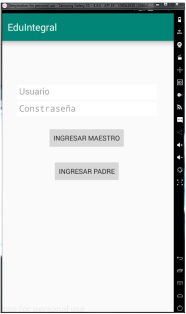
\includegraphics[scale=0.9]{Propuesta_Plantilla_Tesis_LaTeX_UAG/imagenes/eduintegral.png}
                \caption{Eduintegral}
                \label{fig:eduintegral}
            \end{figure}


    \section{Aplicaciones comerciales}
        
        Dentro del ámbito escolar también se encuentran aplicaciones comerciales las cuales al detectar la problematica que existe acerca del desempeño estudiantil y de la desconexión del núcleo familiar con respecto a la escuela, intentan tambien proveer una solución, trayendo consigo multiples funcionalidades y un sistema de mayor competencia, lo cual se cree es algo bueno para la causa de los alumnos. A continuación se presentan algunas de las aplicaciones móviles más relevantes del mercado.
    
        
        \subsection{Schoolway}
        
            Disponible para teléfonos inteligentes con sistema operativo Android y iOS, la aplicación se puede descargar de manera gratuita contactando directamente al desarrollador, dado que ya no se encuentra disponible en la Play Store de momento, la escuela que este interesada en la aplicación tiene que pagar una suscripción para poder usarla \cite{schoolway}. \\ La aplicación es capaz de conectar alumnos, escuela y a los padres de familia dentro de la misma comunidad estudiantil. Da avisos generales utilizando notificaciones push ilimitadas, que inclusive pueden ser programadas con antelación, se pueden crear grupos dentro de la aplicación. \\ La administración y el acceso a la base de datos se considera que es cerrada dado que el control total de la aplicación es solo por parte del desarrollador. La siguiente imagen muestra el logo de la aplicación firmado por su desarrollador (ver figura 2.4).

            \begin{figure}[H]
                \centering
                
\includegraphics[scale=3.0]{Propuesta_Plantilla_Tesis_LaTeX_UAG/imagenes/schoolway.png}
                \caption{Jostens schoolway}
                \label{fig:schoolway}
            \end{figure}


        \subsection{Edmodo for parents}
        
            Aplicación móvil disponible para teléfonos inteligentes con sistema operativo Android y iOS, la cual se puede descargar de manera gratuita desde las tiendas digitales oficiales. La antigua imagen de edmodo se puede apreciar en la siguiente imagen (ver figura 2.5).
        
            \begin{figure}[H]
                \centering
                
\includegraphics[scale=0.2]{Propuesta_Plantilla_Tesis_LaTeX_UAG/imagenes/edmodo.jpeg}
                \caption{Edmodo for parents}
                \label{fig:edmodo}
            \end{figure}
        
            La aplicación actual cuenta con más de 10 millones de descargas en la Play Store, la aplicación pone a disposición del maestro el poder avisar a los padres de familia acerca de tareas, presentaciones y anuncios de maestros. Los padres de familia son más aparte capaces de consultar la información sobre calificaciones y actividades del alumno. La administración y el acceso a la base de datos se considera cerrado dado que esa parte de la aplicación solo puede ser manejada por el desarrollador. La aplicación opera sobre un modelo freemium lo cual significa que parte del uso es gratuito pero para obtener algunas funcionalidades se tiene que pagar una cuota. Edmodo rediseño su imagen en general, creando a su vez un nuevo logo (ver figura 2.6) \cite{edmodo}.
        
            \begin{figure}[H]
                \centering
                
\includegraphics[scale=0.2]{Propuesta_Plantilla_Tesis_LaTeX_UAG/imagenes/edmodo.png}
                \caption{Edmodo for parents nuevo logo}
                \label{fig:edmodo}
            \end{figure}


        \subsection{ClassDojo}
        
            ClassDojo se encuentra disponible para dispositivos móviles con sistema operativo Android y iOS, la aplicación se puede descargar en la tienda digital de dichos sistemas operativos. La aplicación aclama que el uso es gratuito por siempre para maestros que la quieran usar, más sin embargo para poder acceder al contenido premium se requiere pagar por el mismo, más aparte cuenta con un servicio de pago mensual con algunas opciones extra. \\ ClassDojo cuenta con mas de 10 millones de descargas en la Play Store, siendo esta una aplicación muy popular (ver figura 2.7) \cite{classdojo}. 
            
            \begin{figure}[H]
                \centering
                
\includegraphics[scale=0.2]{Propuesta_Plantilla_Tesis_LaTeX_UAG/imagenes/classdojo.jpg}
                \caption{ClassDojo}
                \label{fig:classdojo}
            \end{figure}
            
            La aplicación cuenta con una especie de salón de clases virtual utilizando la nube, al salón virtual pueden ser invitados los padres de familia de los alumnos que ya se encuentren dentro. A los integrantes del salón la aplicación les permite compartir fotos, videos y anuncios al mismo salón. La administración y acceso a la base de datos es permitida sólo por el desarrollador \cite{classdojo}. 
    
    
        \subsection{Remind-School Communication}
        
            La aplicación Remind-School Communication se encuentra disponilbre para teléfonos inteligentes con sistema operativo Android y iOS, esta se puede descargar de manera gratuita desde las tiendas digitales oficiales. \\ Ofrece a los maestros una forma sencilla y segura para enviar SMS a estudiantes y padres de familia, la aplicación aclama que es segura porque mantiene de forma segura los números de telefono. También permite a maestros, monitores o administradores el envio de recordatorios, tareas, actividades, evaluaciones y mensajes motivadores. La administración de la aplicación y el acceso a la base de datos es por parte del desarrollador por lo cual el acceso es cerrado. \\ La descarga y el uso básico de la aplicación es gratuito, también cuenta con un plan premium el cuál es de paga.La aplicación cuenta con mas de 10 millones de descargas desde la Play Store (ver figura 2.8) \cite{remind}.
            
            \begin{figure}[H]
                \centering
                
\includegraphics[scale=0.4]{Propuesta_Plantilla_Tesis_LaTeX_UAG/imagenes/remind.png}
                \caption{Remind-School Communication}
                \label{fig:remind}
            \end{figure}


    \section{Discusión de otras aplicaciones}
    
    Revisado las aplicaciones analizadas se pueden inicialmente dividir en aplicaciones comerciales y apliciones no comerciales, lo cual indica ya en si una diferencia en cuanto a que unas aplicaciones limitaran la funcionalidad que se otorga ha no ser de que se realice un pago mensual mientras que las aplicaciones no comerciales otorgan todas las funcionalidades de manera completa y sin costo, aunque tambien cabe mencionar que las apliciones comerciales mostraron generalmente tener muchas funciones extras. \\ Se puede deducir que todas las apliciones si llegan a proporcionar en cierto grado una comunicación entre padres de familia y maestros, haciendo uso de las notificiones push proporcionadas por el sistema y de grupos generados en base a los grupos escolares de las escuelas. La mayoría de las aplicaciones se encuentran disponibles al momento de realizar este proyecto, tambien cabe mencionar que se observo que el uso de las aplicaciones comerciales sobre pasa por mucho el uso de las aplicaciones no comerciales, dando cifras por millones de usuarios de diferencia, aunque en el caso de Eduintegral, esta todavía no se encuentra dispobile al público. \\ Aunque para el caso de estudio de este proyecto cabe mencionar que la cantidad de usuarios activos o de paga no es relevante. El punto negativo de todas las aplicaciones comerciales es el cobro de una cuota mensual para el uso de las funcionalidades premium o para acceder a contenido especial. También se observo que con las aplicaciones comerciales no se tiene autorizado por parte de los desarrolladores el acceso a las bases de datos de las aplicaciones, también la administración de las mismas aplicaciones se vio mermada por esta situación dado que esta cerrada para terceros. \\ La seguridad y privacidad que puede tener la información de todos los usuarios por parte de las aplicaciones comerciales es una incognita dado que los desarrolladores de las mismas mantienen en privado dicha información y no se dan más detalles.
    Finalmente, se puede decir que el enfoque de las aplicaciones comerciales va más dirigido a las actividades y tareas llevadas en el salón de clases que en mejorar la comunicación entre padres de familia y maestros. Dadas todas estas caracteristicas y detalles observados durante la investigación se generó la siguiente tabla comparativa, mostrando de manera clara y concisa todos los puntos evaluados según el objetivo de este trabajo (ver tabla 2.1) \cite{eduintegral}.
        
        \begin{table}[H]
            \centering
            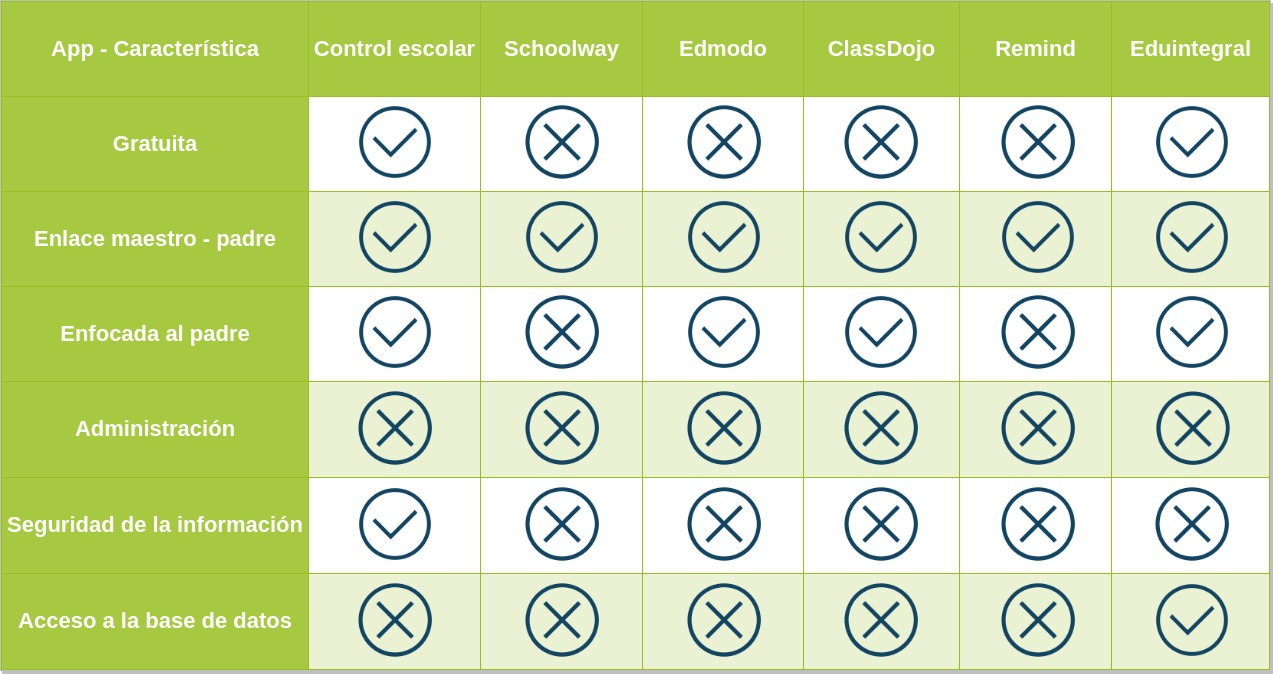
\includegraphics[scale=0.3]{Propuesta_Plantilla_Tesis_LaTeX_UAG/imagenes/tabla_comparativa_de_aplicaciones.jpg}
            \caption{Tabla comparativa de aplicaciones}
            \label{tab:comparativa}
        \end{table}
        
        \begin{itemize}
            \item \textbf{Gratuita:} Se refiere a si la aplicación se puede descargar y usar de manera gratuita por todos los involucrados
            
            \item \textbf{Enlace maestro-padre:} Indica si la aplicación logra la comunicación directa, total o parcialmente, entre padres de familia y el maestro
            
            \item \textbf{Enfocada al padre:} Nos dice si la aplicación está enfocada, diseñada y dirigida para uso especı́fico del padre de familia, tomando en cuenta sus requerimientos más importantes sobre otras funciones que no sean tan necesarias \cite{eduintegral}
            
            \item \textbf{Administración:} Describe si la aplicación permite ser administrada y adaptada a las necesidades particulares de las escuelas
            
            \item \textbf{Seguridad de la información:} Analiza si la información que se propociona a la aplicación y por ende al desarrollador está resguardada de manera segura, si se menciona en dónde será almacenada, cómo se resguarda y por último si el uso que se le dará a dicha información es mencionado
            
            \item \textbf{Acceso a la BD:} Muestra si al usar la aplicación podemos tener acceso a los datos recabados en la base de datos para efectos de análisis y/o estadı́sticos o si en todo caso podemos resguardar nuestros propios datos en una base de datos local.
            
        \end{itemize}
    % Capitulo 02
        
        \chapter{Propuesta y diseño}
        %Capítulo 3

Este trabajo busca cumplir con la propuesta original realizada por Eduintegral, al crear una aplicación móvil la cual búsca crear, manetener y fortalecer el vinculo entre padres de familia y maestros. \\ Más aparte esta propuesta búsca ampliar la forma en la que se almacenan los datos, cumplir con la parte de administración de la aplicación y más aparte considerar un flujo seguro en el almacenamiento de los datos generados por la aplicación. \\ El objetivo primordial de Eduintegral sigue siendo el asegurar un buen desempeño del alumno basandonos en la mejora de la comunicación entre el maestro y los padres de familia, los cuales al tener una buena comunicación pódran detectar y solucionar problematicas en el desempeño de los alumnos.

\section{Modelo conceptual}
    
    El modelo conceptual del proyecto de mejora sobre Eduintegral se basa a partir de las caracteristicas definidas en la sección previa (ver sección 2.3). \\ El siguiente diagrama conceptual muestra de manera teórica como se desea que se comporte el sistema de manera generalizada (ver figura 3.1).
    
    \begin{figure}[H]
        \centering
        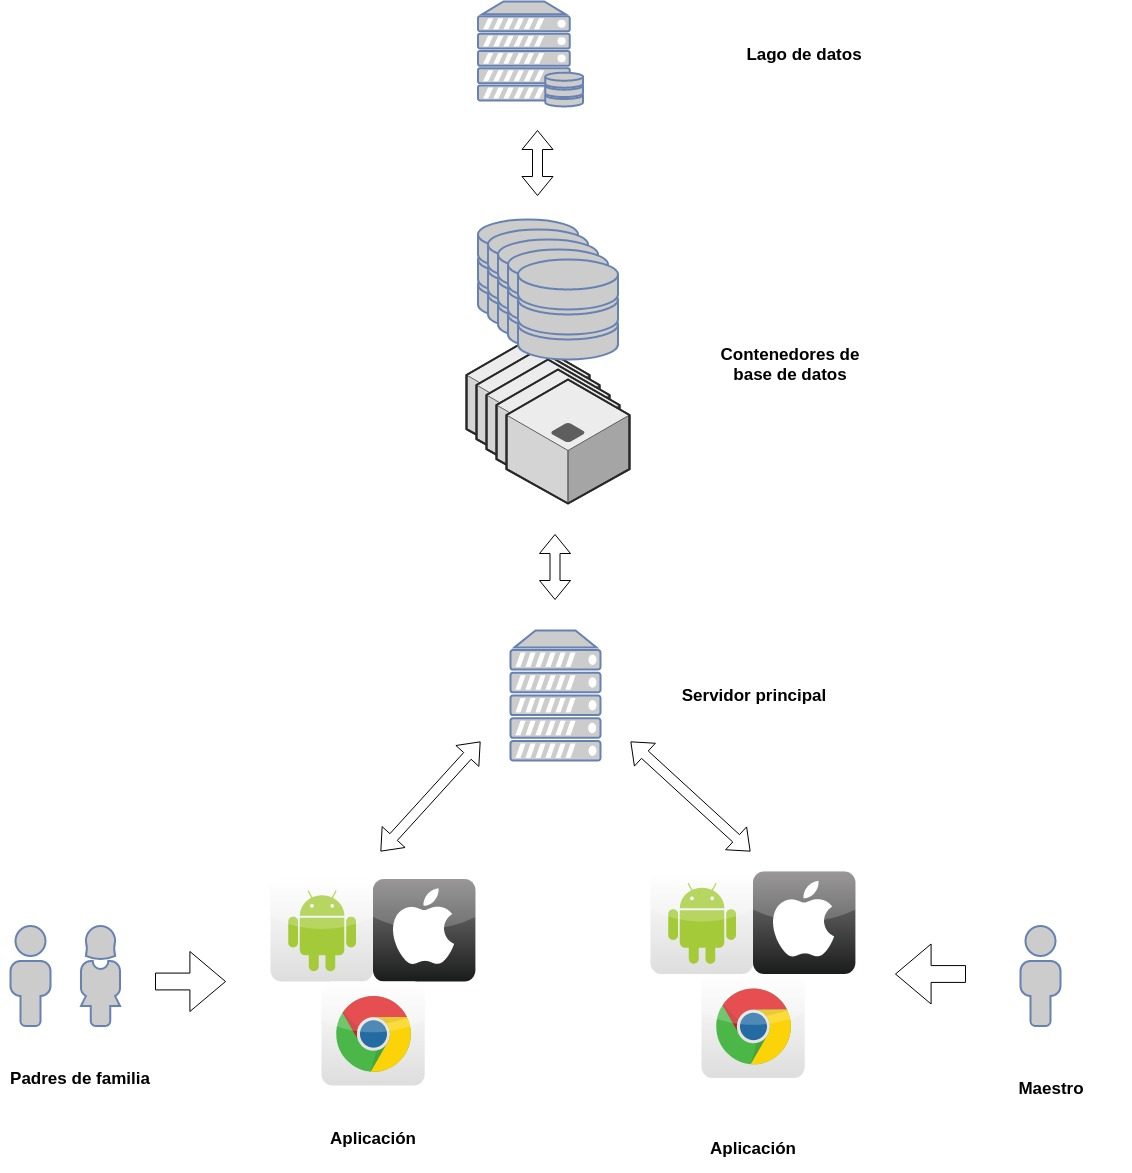
\includegraphics[scale=0.3]{imagenes/arquitectura_propuesta.jpg}
        \caption{Diagrama modelo conceptual}
        \label{fig:diagramamodeloconceptual}
    \end{figure}
    
    \begin{itemize}
    
        \item \textbf{Maestro:} Captura las calificiones de alumnos, registra la asistencia y ausencias de los alumnos, manda reportes a los padres de familia si los alumnos incurren en faltas
        
        \item \textbf{Padres de familia:} Consultan las calificaciones, ausencias y asistencias de sus hijos, recibe notificaciones por parte de los maestros
        
        \item \textbf{Aplicación:} Aplicación móvil y aplicación web capaz de servir como medio de consulta y captura de las calificaciones, asistencias y ausencias, tambien es capaz de manejar el envio de notificaciones de maestros a padres de familia
        
        \item \textbf{Servidor principal:} Es el servidor físico el cual albergara los contenedores de bases de datos, en el tambien se almacerá de momento el lago de datos
        
        \item \textbf{Contenedores de base de datos:} Estructura propuesta de manejo de contenedores con bases de datos
        
        \item \textbf{Lago de datos:} Lago de datos que almacenara todos los datos generados por el sistema
        
    \end{itemize}
    
    
\section{Base de datos}
    
    La base de datos es una de las partes principales de la arquitectura de este proyecto dado que esta tendra la estructura requeridad para almacenar todos los datos generados por la aplicación. \\ Se pretende cambiar completamente el diseño de la base de datos para que esta puede manejar mayores cantidades de datos y a su vez prepararla para soportar de manera eficiente la cantidad de consultas que se espera por todos los maestros y padres de familia de las escuelas. \\ Las caracteristicas principales encontradas para establecer esta propuesta sobre el diseño de la base de datos son:
    
    \begin{itemize}
        \item Se requiere tener registro de todos los usuarios capaces de acceder a la aplicación, un dato importante a considerar es que se tienen que diferenciar maestros de padres de familia
        
        \item Toda la información personal que rodea al alumno dentro del ámbito escolar, dicese de datos como el nombre, grado y grupo, ciclo escolar que esta cursando
        
        \item Se considera importante el tener registro sobre las asistencias y ausencias de los alumnos, teniendo en cuenta que estas se pueden dar por materias
        
        \item Es necesario conocer cuales son las materias impartidas en una especifica escuela
        
        \item Para la comunicación del padre de familia y el maestro se concentraran los reportes y los tipos de reportes que se generen
        
        \item Las calificaciones del alumno se mantendran registradas dado que es un indicador importante sobre el demsempeño estudiantil
        
        \item Los datos de maestros y padres de familia serán ligados a los datos de los alumnos 
        
        \item Se considera relevante almacenar la información pertinente de las escuelas en las que se encuentran laborando los maestros y por ende estudiando los alumnos
        
    \end{itemize}
    
    El siguiente diagrama (ver figura 3.2) muestra el diseño original de la primer base de datos propuesta para Eduintegral \cite{eduintegral}, más el diseño extendido de la base de datos propuesta en este trabajo, en la cual se consideran otras entidades adicionales que se cree ayudarán a tener la mayor cantidad de datos relevantes.
    
    \begin{figure}[H]
        \centering
        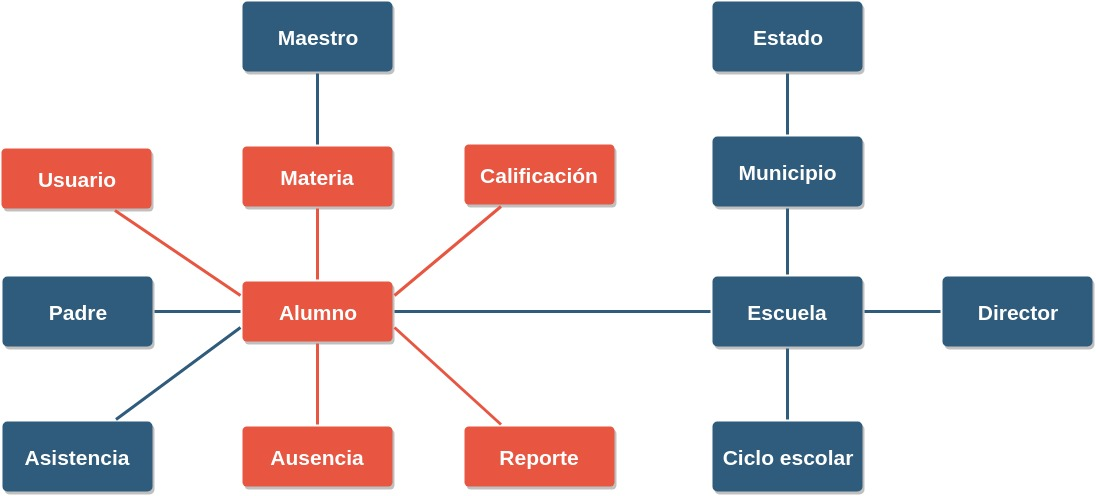
\includegraphics[scale=0.4]{Propuesta_Plantilla_Tesis_LaTeX_UAG/imagenes/base_de_datos_2.jpg}
        \caption{Diagrama de base de datos}
        \label{fig:diagramabasededatos}
    \end{figure}
    
    \begin{itemize}
    
        \item \textbf{Diagrama color rojo:} Diseño de base de datos original generado para el desarrollo de Eduintegral \cite{eduintegral}
        
        \item \textbf{Diagrama color verde:} Diseño de base de datos que contiene el diseño original propuesto más entidades que expanden la capacidad de almacenamiento de datos
        
    \end{itemize}    % Capitulo 03
        
        \chapter{Implementación y pruebas}
        %Capítulo 4    % Capitulo 04
        
        \chapter{Discusión, conclusiones y trabajo futuro}
        %Capítulo 5    % Capitulo 05
        
        
        \bibliographystyle{ieeetr} % Formato de la IEEE
        \bibliography{bibliografia/articulos.bib,bibliografia/libros.bib,bibliografia/misc.bib}
    
    \end{document}
%-----------------------------------------------------------%